\section{Datenverarbeitung}\label{db}

Eine gehostete Datenbank eröffnet unserem Wetter-API System viele weitere Möglichkeiten. Neben System User Informationen der Messaging Oriented Middleware RabbitMQ ,  können die empfangenen Wetterdaten kontinuierlich abgespeichert werden. Die hinterlegten Daten können nun für eine Reihe von Statistiken und Auswertungen genutzt werden und bieten außerdem den Vorteil  den künftigen Ressourceneinsatz und die Skalierung effizienter zu gestalten. 
In diesem Kapitel wird eines passenden Datenbank  beschrieben. Da das Testen eines skalierbaren Datenbankservices in der Regel sehr teuer ist, werden einige Funktionalitäten nur in der Theorie beschrieben. Dennoch lässt sich der Nutzen eines Datenbankkonzepts klar herausstellen.
Zur Speicherung der Datensätze wird ein relationales Datenbankschema auf MYSQL Basis verwendet. Gehostet wird über den Amazon Web Service Dienst RDS. Für eine einfache Implementierung und Verwendung der Datenbank in den Systemmodulen CEP und MQTT (RabbitMQ) wird eine JDBC API Schnittstelle zur Verfügung gestellt.

\subsection{Datenbankschema}

\textbf{System User und vHost ER Modell}
Das Datenbankschema lässt sich in 2 verschiedene Bereiche unterteilen. Neben einer Speicherstruktur für die eingehenden Wetterdaten, lassen sich auch User Accountinformationen der RabbitMQ abspeichern. In Abbildung \ref{img:DBSchemaSystemUser} ist das Schema der Tabellenkonstellationen für die Speicherung der SystemUser zu sehen.
\begin{figure}[htbp]
	\centering
	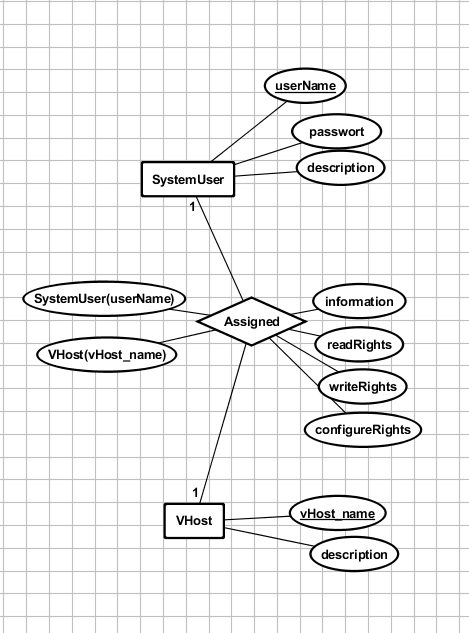
\includegraphics[width=0.5\textwidth]{Bilder/DBSchemaSystemUser.png}
	\caption{Datenbank ER Modellierung - RabbitMQ System Data}
	\label{img:DBSchemaSystemUser}
\end{figure} 
Die Tabelle SystemUser  beinhaltet die Login Credentials und die Tabelle vHost lässt die Sicherung der RabbitMQ Informationen zu. 
Die n:m Beziehung zwischen System Usern und vHost wird in der Tabelle Assigned abgebildet. Hier lassen sich auch die jeweiligen Berechtigungen read, write und configure des Users auf der RabbitMQ Instanz hinterlegen.

\textbf{Wetter Daten ER Modell}
Damit die eingehenden Daten der Wetter-API  korrekt abgelegt werden können, sind Stammdaten in der Datenbank gepflegt. Neben den zur Verfügung stehenden Städten in der Tabelle City, werden auch die Standardwetterdaten (Tabelle DeaultWeather) aus der verwendeten Wetter-API hinterlegt. Jedes eingehende  Wetterdatenobjekt ist einer Stadt zugeordnet und referenziert ein DefaultWeather Eintrag.
Die User unserer Systemlösung können ebenfalls in der Datenbank gespeichert werden. Die Tabelle Subscribe beinhaltet die n:m Referenzen von Usern, welche bestimmte Städte beziehungsweise deren Wetterdaten abonniert haben. Jeder Eintrag in der Tabelle Subscribe besitzt zudem das Datum der Aktivierung des Abonnements. Abbildung \ref{img:DBSchemaWetterDaten} visualisiert das ER Modell der Wetterdatenspeicherung.
\begin{figure}[htbp]
	\centering
	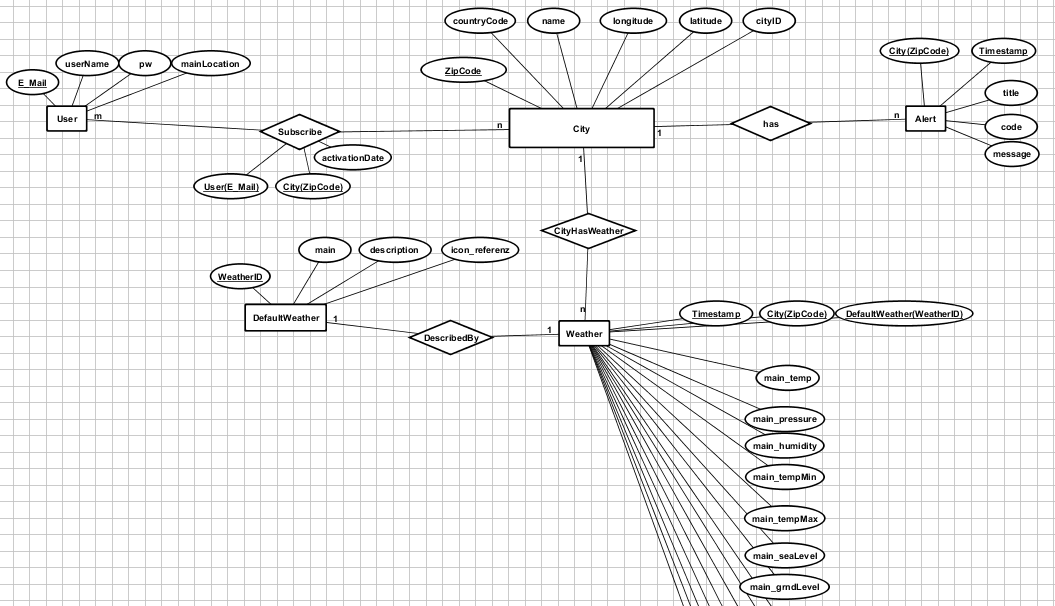
\includegraphics[width=0.5\textwidth]{Bilder/DBWetterDaten.png}
	\caption{Datenbank ER Modellierung - Wetter Daten Modellierung}
	\label{img:DBSchemaWetterDaten}
\end{figure} 
Die Complex Event Processing Engine, kurz CEP, errechnet anhand der eingehenden Wetterdaten verschiedene Benachrichtigungen (Alerts), welche über die MOM als Topic an die User verteilt werden. In der Datenbank können diese Alerts in Abhängigkeit der betroffenen Stadt gespeichert werden.

\subsection{Datenbank – JDBC Schnittstelle}
Der Zugriff und die Verwaltung der Datensätze nach dem, im vorherigen Kapitel beschrieben, Datenschema, ist in der Java Klasse CadWeatherSystemDatabaseAPI realisiert. Diese Klasse lässt sich in alle Teilmodule unseres Gesamtsystems implementieren und bietet eine Schnittstellefunktionalität zur Verwendung der Datenbankinstanzen. In den Java Methoden, werden die MYSQL Kommunikationssatetments codiert als String über ein connection Objekt auf der Datenbank ausgeführt. Grundsätzlich stehen INSERT Operationen für alle Tabellen, sowie diverse SELECT Abfragemöglichkeiten zur Verfügung. Ziel dieser Struktur ist eine simple, vereinheitlichte Methodik zur Benutzung der Datenbankinstanzen.
Der Konstruktor der Klasse gibt dem Entwickler die Möglichkeit ein MYSQL Datenbankobjekt in die Schnittstelle einzubinden.

In der nachfolgenden Tabelle sind alle derzeit programmierten Methoden aufgelistet.
Die INSERT  Methoden liefern das Feedback der Datenbankoperation in einem String zurück. Die Rückgabe ResultSet der select-Methoden beinhaltet die gefunden Datentupel der Abfrage.

{\bf GENERAL DB}
\begin{itemize}
\item String  checkDatabaseConnection()
\item java.sql.Connection getConnection()
\item setConnection(java.sql.Connection  databaseConnection)
\end{itemize}

{\bf CEP DB - INSERT}
\begin{itemize}
\item String insertDefaultWeather(int WeatherID, String main, String description, String iconReferenz)
\item String insertCity(int ZipCode, String cityName, Double logitude, Double latitude, int cityID)
\item String insertUser(String EMail, String userName, String passwort, int mainLocation)
\item String insertSubcribe(String EMail, int ZipCode)
\item String insertAlert(int ZipCode, Timestamp timestamp, String title, String code, String message)
\item String insertWeather(Timestamp TimeStamp, int ZipCode, int WeatherID, 
				double mainTemp, double mainPressure, double mainHumidity, double mainTempMin,
				double mainTempMax, double mainSeaLevel, double mainGrndLevel,
				String windDirection, double windSpeed, double windDeg, String cloudsDesc, double rain3h, 
				double snow3h, 
				Timestamp sysSunset, Timestamp sysSunrise)
\end{itemize}
\newpage
{\bf CEP DB - SELECT }
\begin{itemize}
\item ResultSet selectUserByMail(String userEMail)
\item ResultSet selectCityByZipCode(int cityZipCode)
\item ResultSet selectDefaultWeatherByID(int defaultWeatherID)
\item ResultSet selectAllWeatherByCityZipCode(int cityZipCode)
\item ResultSet selectWeatherByCityAndDay(int cityZipCode, Timestamp weatherDay)
\item ResultSet selectWeatherByCityAndTimePeriod(int cityZipCode, Timestamp fromDate, Timestamp toDate) 
\item ResultSet selectSubscribeByUser(String userEMail)
\item ResultSet selectSubscribeByCity(int ZipCode)
\item ResultSet selectUserPwByEMail(String EMail)
\end{itemize}

{\bf RabbitMQ DB - Insert }
\begin{itemize}
\item String insertSystemUser(String userName, String password, String additionalDescription)
\item String insertVHost(String vHostName, String additionalDescription)
\item String insertAssigned(String systemUserUserName,String vHostName, String additionalInformation, boolean readRights, boolean writeRights, boolean configureRights);
\end{itemize}

{\bf RabbitMQ DB - SELECT }
\begin{itemize}
\item ResultSet selectVHostAll()
\item ResultSet selectSystemUserAll()
\item ResultSet selectSystemUserByUserName(String userName)
\item ResultSet ResultSet selectAssignedAll()
\end{itemize}



\subsection{Auswertungen und Nutzen der Datenbankspeicherung}
Die Datensätze können vielseitig genutzt werden. Zum einen hält die CEP Komponente unseres Systems die empfangen Wetterdaten der MOM bzw. der Wetter-API nur temporär. Gleiches gilt für erzeugte Benachrichtigungen in Form von Alerts.
Durch eine Sicherung in der Datenbank stehen die Wetterdaten unabhängig vom Status der CEP persistent zur Verfügung. 
Des Weiteren können verschiedene Auswertungen der Datensätze weitere Erkenntnisse bringen. 

\textbf{Wetter-API User}
Durch die Protokollierung der Alerts lassen sich Statistiken über die Ereignisse und deren Verteilung aufstellen. Daraus könnten wir für die User beispielsweise Vorabwarnungen zukommen lassen. Außerdem könnte man den Usern auf lange Sicht gesehen Wettervergleiche bzw. Wetterentwicklungen bereitstellen.

\textbf{Cloud System Analyse}
Mithilfe des gespeicherten Datums der Aktivierung  von User Abonnements zu den jeweiligen Städten, lässt sich auch eine Prognose für unser System erstellen. Je nach Modell der Verteilung der gehosteten Komponenten unseres Systems  können wir aus den Datensätzen abschätzen, wie sich die Last auf unserem System entwickelt. 
Diese Prognosen können für eine Kostenabschätzung des Cloudsytsem wertvoll sein, um Ressourcen effizient einzusetzen und damit verbundene Kostenpunkte besser vorherzusagen.
Selbstverständlich ist der größte Vorteil einer Cloudlösung das dynamische Reagieren auf verschiedene Lastverhalten. Dennoch ist es im Rahmen von Businessmodellen notwendig zu wissen, welche Kosten an welcher Stelle entstehen beziehungsweise geplant werden können.

\subsection{AWS RDS Datenbankverfügbarkeit}
In Bezug auf die Performance spielt bei der Datenbank nur die Anzahl der CEP Calls eine Rolle. Dies führt je nach Szenario und Wetterveränderungen unterschiedlich viele I/O Operationen aus. Dennoch würde unser Wetter-API System selbst bei extrem hohen Userzahlen keine Datenlast liefern, welche die Datenbank an ihre Grenze bringen könnte. Das Bottleneck unseres Systems sind die Instanzen der CEP. Im Rahmen unseres Projektes ist die Skalierung des Datenbank Services nicht eingerichtet, da zusätzliche oder skalierte Datenbankinstanzen mit hohen Kosten verbunden sind. Die benötigten Konfigurationen sind nicht im Umfang des AWS Trialkontingents enthalten . Ganz wichtig ist die Tatsache, dass das Starten einer weiteren Instanz das kostenlose Kontigent an Ressourcen aufhebt. Aus eigener Erfahrung wissen wir, wie sich ein solches Szenario zu einer gewissen Kostenfalle entwickeln kann.
An dieser Stelle sollen dennoch die Möglichkeiten der Datenbankverfügbarkeit in Bezug auf den AWS RDS Dienst beschrieben werden.

\textbf{Vertikale Skalierung}
Die Datenbank empfängt viele write-Operationen, weshalb eine vertikale Skalierung in unserem Fall der beste Ansatz wäre. Amazon bietet in seinem Service EC2/RDS (Relationale Datenbank Services) automatische Skalierungsoptionen an. So lassen sich verschiedene Monitoring Parameter (z.B. CPU Auslastung) einstellen, welche beim Erreichen eines Grenzwertes automatisch weitere Kapazitäten zur Verfügung stellt. Der Datenbankinstanz können je nach genutzer Datenbankengine bis zu 32 vCPU's mit 244GB RAM uns bis zu 64TB Datenspeicher zugeschaltet werden. Ein minimaler Nachteil ist eine kurze Downtime Phase in der die neuen Ressourcen eingebunden werden. Es gehen aber keine gespeicherten Daten verloren, sodass man in die Write Operationen der CEP im internen Speicher der CEP halten und bei erneuter Datenbankverfügbarkeit an den RDS Dienst übergeben könnte.

\textbf{Horizontale Skalierung}
Eine horizontale Skalierung eignet sich vor allem bei Applikationen mit einem hohen Anteil an read-Operationen. Hierfür kann man beispielsweise den Amazon Container Service (EC2) konfigurieren. Zum Beispiel könnte man bei einem gewissen Lastverhalten einen Dockercontainer verwenden und eine weitere Instanz aufzuziehen.
Eine weitere Möglichkeit für eine horizontale Skalierung, sind READ Replica Objekte. Ein READ Replica Objekt bildet den Aufbau und den Inhalt einer Datenbankinstanz ab, womit READ Operationen von Insert Operationen getrennt und verteilt werden können. Damit erreicht man eine große Steigerung der Performance von Write-Operationen auf der Datenbank. Der RC2 Task zur Generierung eines READ Replica Objekts und das zugehörige LoadBalancing benötigt eine weitere Instanz, was nicht im AWS Trialkontingents enthalten ist und somit nicht eingerichtet wurde.

\textbf{Ausfallsicherheit}
Für die Ausfallsicherheit bietet der AWS RDS Dienst die Option Multi-AvailabilityZone. Wenn die Option aktiviert wird, erstellt Amazon eine synchronisierte Datenbankinstanz in einer anderen Region beziehungsweise in einem anderen Rechenzentrum. Beim Ausfall der aktiven Datenbankinstanz wird innerhalb einer Minute die synchrone Datenbankinstanz zugeschaltet und das DNS angepasst, damit sich aus Applikationssicht nichts verändert.
Des Weiteren wird in einem definierbaren Zeitintervall ein BackUp der Datenbank erstellt.


\subsection{12 Faktor App}\label{12FactorApp}
In diesem Absatz wird dargestellt, ob und wie die Anforderungen umgesetzt wurden.


\begin{table}[!ht]
  \centering
    \begin{minipage}{17cm}
      \centering
      \begin{tabular}{*{3}{|l|p{3.0cm}|p{7.0cm}}}\hline
      \multicolumn{4}{|c|}{\cellcolor[RGB]{200,200,200}Validierung nach "12 Faktor APP"} \\\hline
     \textbf{ID}&\textbf{Anforderung}&\textbf{Validierungs Element}&\textbf{Erfüllt}\\\hline
      1.&Codebase&Andere Komponenten sind nur für das Testszenario da. Deployment verschiederner Versionen über Repo möglich&Ja\\
      \hline
     2.&Abhängigkeiten&Zugriff auf die MYSQL Datenbank des AWS RDS Dienstes sind in einer API Klasse definiert und isoliert&Ja\\
     \hline
     3.&Konfiguration&Die Credentials für die Datenbank API Nutzung sind in den Umgebungsvariablen eingetragen&Ja\\
     \hline
     4.&Unterstützende Dienste& &Nein\\
     \hline 
     5.&Build, release, run& &Nein\\
     \hline
     6.&Prozesse& &Nein\\
     \hline
      \end{tabular}
   \caption{Validierung der Datenverarbeitung nach "12 Faktor APP"}\label{tab:AnforderungenDB}
    \end{minipage}
\end{table}
\newpage
\begin{table}[h]
  \centering
    \begin{minipage}{17cm}
      \centering
      \begin{tabular}{*{3}{|l|p{3.0cm}|p{7.0cm}}}\hline
      \multicolumn{4}{|c|}{\cellcolor[RGB]{200,200,200}Validierung nach "12 Faktor APP"} \\\hline
     \textbf{ID}&\textbf{Anforderung}&\textbf{Validierungs Element}&\textbf{Erfüllt}\\
     \hline
      7.&Bindung an Ports& &Nein\\
     \hline
      8.&Nebenläufigkeit&Die Skalierung kann über Amazon EC2 erfolgen - Load Balancing oder READ Replica Verteilung von Tasks auf verschiedene Instanzen (Nicht umgesetzt, 		da nicht im AWS Testkontingent enthalten)&Mglich\\
     \hline
      9.&Einweggebrauch&Die Datenbankinstanz kann über AWS Management Console oder das Amazon Comand Line Interface gestoppt und gestartet werden &Teilweise\\
     \hline
     10.&Dev-Prod-Vergleichbarkeit&Mithilfe einer synchronen Datenbankinstanz umsetzbar - Einstellung im AWS Service (Nicht umgesetzt, da nicht im AWS Testkontingent enthalten) &Moeglich\\
     \hline     
     11.&Logs&AWS Monitoring (Enhanced Monitoring) erlaubt Tracking und Analyse von ausgeführten MYSQL Operationen&Ja\\
     \hline
     12.&Admin-Prozesse&&Nein\\
     \hline
      \end{tabular}
   \caption{Validierung der Datenverarbeitung nach "12 Faktor APP"}\label{tab:AnforderungenDB}
    \end{minipage}
\end{table}